\begin{tikzpicture}
\node[inner sep=0,anchor=south west] (im) at (0,0) {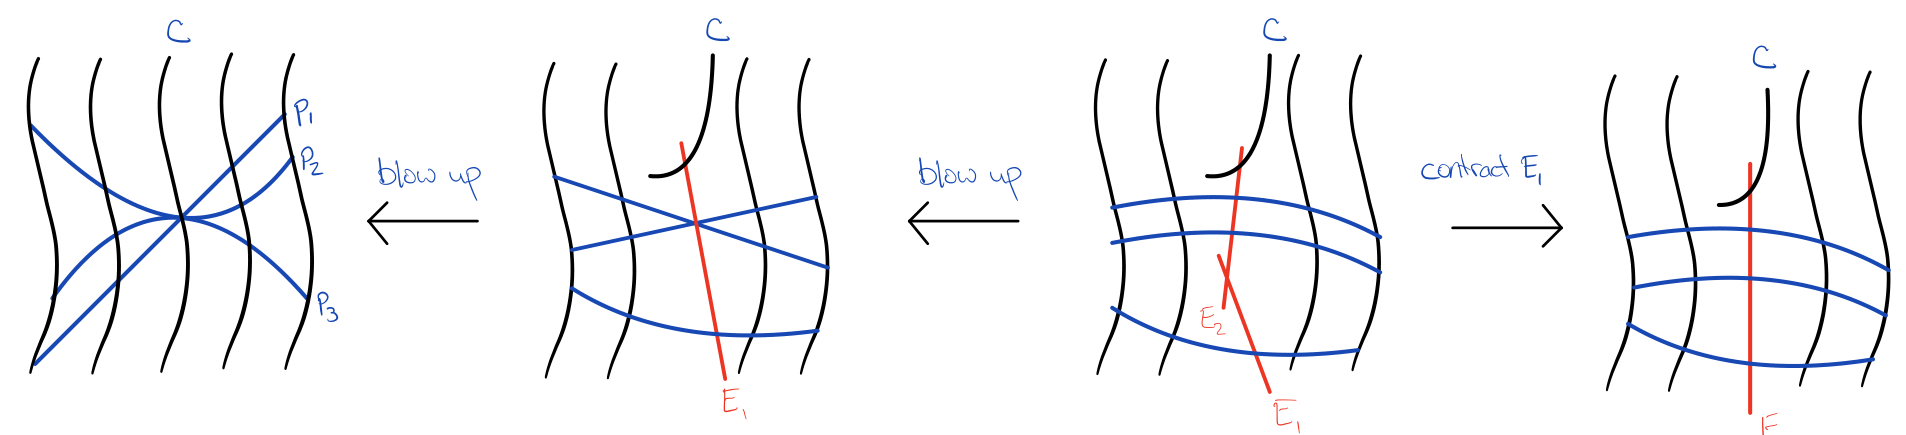
\includegraphics[width=.86\textwidth]{figures/reduction-step5.png}};
\begin{scope}[x={(im.south east)},y={(im.north west)}]
\fill[white] (0.18,0.52) rectangle (0.27,0.73);
\fill[white] (0.46,0.52) rectangle (0.55,0.73);
\fill[white] (0.74,0.52) rectangle (0.83,0.73);
\node[fill=white,inner sep=1pt,font=\scriptsize,text=blue] at (0.223,0.6) {爆破};
\node[fill=white,inner sep=1pt,font=\scriptsize,text=blue] at (0.506,0.6) {爆破};
\node[fill=white,inner sep=1pt,font=\scriptsize,text=blue] at (0.779,0.6) {收缩 $E_1$};
\end{scope}\end{tikzpicture}
